\chapter{Lecture 31 - Polar Coordinates with Angular Symmetry}
\label{ch:lec31}
\section{Objectives}
\begin{itemize}
\item Carry out the separation of variables processes to solve the wave equation in polar coordinates.
\item Show an example implementation in MATLAB.
\end{itemize}
\setcounter{lstannotation}{0}

\section{Wave Equation in Polar Coordinates}
In a few past lectures we have dealt with the wave equation on a line as shown in Equation \ref{eq:lec31-1D-wave}.
\begin{equation}
\frac{\partial^2 u}{\partial t^2} = \alpha^2 \frac{\partial^2 u}{\partial x^2}
\label{eq:lec31-1D-wave}
\end{equation}
This is actually a quite specific articulation of the wave equation, tailored only for a one-dimensional wave.  Waves happen in more than one dimension, however, and we would like to describe those also.  Equation \ref{eq:lec31-wave-general} gives a more general expression of the wave equation using the Laplacian operator that is valid for any number of dimensions over finite or infinite domains.
\begin{equation}
\frac{\partial^2 u}{\partial t^2} = \alpha^2 \nabla^2 u
\label{eq:lec31-wave-general}
\end{equation}
If we specialize the Laplacian operator for 1D Cartesian coordinates then we recover Equation \ref{eq:lec31-1D-wave}

\newthought{In this lecture} we will solve the wave equation in polar coordinates.  Specializing the Laplacian for polar coordinates and inserting into the wave equation gives us:
\begin{equation}
\frac{\partial^2 u}{\partial t^2} = \alpha^2 \left(\frac{\partial^2 u}{\partial r^2} + \frac{1}{r}\frac{\partial u}{\partial r} + \frac{1}{r^2}\frac{\partial^2 u}{\partial \theta^2} \right)
\label{eq:lec31-wave-eqn-polar}
\end{equation}
We will use this equation to model radial vibrations in a circular membrane for which the membrane is fixed (no displacement) all around the periphery at $r=c$.  We will also assume that the initial displacement and velocity of the membrane are functions of radius only.  Because this boundary condition and both initial conditions are constant for all angular positions, we should expect that \emph{the solution} will also be constant for all angular positions; in particular, we expect $\sfrac{\partial u}{\partial \theta}$ and $\sfrac{\partial^2 u}{\partial \theta^2}$ to equal zero.\sidenote[][-1.5cm]{Conversely, if \emph{either} the boundary or initial conditions were a function of angular position, $\theta$, this assumption would not be true and we would need to use the full form of the wave equation in polar coordinates given in equation \ref{eq:lec31-wave-eqn-polar}.} The boundary value problem for this is given below.
\begin{table}
\begin{tabular}{l l}
$\substack{\text{Governing} \\\text{Equation}}: $& $\frac{\partial^2 u}{\partial t^2} = \alpha^2 \left(\frac{\partial^2 u}{\partial r^2} + \frac{1}{r}\frac{\partial u}{\partial r}\right), \ \ \alpha > 0, \ 0<r<c, \ t>0$  \\
& \\
$\substack{\text{Boundary} \\ \text{Condition}}: $& $u(c,t) = 0, \ \ t>0$\\
& \\
$\substack{\text{Initial} \\ \text{Conditions}}: $ & $u(r,0) = f(r), \ \ u_{t}(r,0) = g(r), \ \ 0<r<c $ \\
\end{tabular}
\end{table} 

\vspace{0.25cm}

\newthought{We will solve} this boundary value problem using separation of variables.

\vspace{0.25cm}

\noindent\textbf{Step \#1:} Assume a product solution.
\begin{equation*}
u(r,t) = F(r)G(t)
\end{equation*}

\vspace{0.25cm}

\noindent\textbf{Step \#2:} Insert the product solution into the governing equation.
\begin{align*}
\frac{\partial^2 }{\partial t^2}\left(F(r)G(t)\right) &= \alpha^2 \left[\frac{\partial^2}{\partial r^2}\left(F(r)G(t) \right) + \frac{1}{r}\frac{\partial}{\partial r}\left(F(r)G(t)\right) \right] \\
FG_{tt} &= \alpha^2 \left(F_{rr}G + \frac{1}{r}F_rG \right)
\end{align*}

\vspace{0.25cm}

\noindent\textbf{Step \#3:} Separate variables.

\begin{align*}
\frac{FG_{tt}}{\alpha^2 FG} &= \frac{\alpha^2 \left(F_{rr}G + \frac{1}{r}F_rG \right)}{\alpha^2 FG} \\
\frac{G_{tt}}{\alpha^2 G} &= \frac{F_{rr} + \frac{1}{r}F_r}{F} = -\lambda
\end{align*}
So the separated equations are:
\begin{align*}
F_{rr} + \frac{1}{r}F_r + \lambda F &= 0 \\
G_{tt} + \alpha^2 \lambda G &= 0
\end{align*}

\vspace{0.25cm}

\noindent\textbf{Step \#4:} Apply boundary conditions to find non-trivial solutions.

\vspace{0.25cm}

\noindent We will take a short-cut here by assuming that the separated solution $G(\theta)$ must be periodic and, having done this before, we know that this implies $\lambda >0$.  Setting $\lambda = \nu^2, \ \nu>0$, we get:
\begin{align*}
G_{tt} + \alpha^2 \nu^2 G &= 0 \\
r^2F_{rr} + rF_r + \alpha^2\nu^2 F &= 0
\end{align*}
where, to put the equation for $F(r)$ in a more familiar form, we multiplied through by $r^2$.  The general solution for both equations is:
\begin{align*}
F(r) &= c_1J_0(\nu r) + c_2 Y_0(\nu r) \\
G(t) &= c_3\cos(\nu \alpha t) + c_4 \sin(\nu \alpha t)
\end{align*}

\newthought{In the $r$-coordinate} we have only one explicit boundary condition, but there is another condition of which we must always be mindful, particularly in polar coordinates when $r=0$ is part of the domain; that is that $\lim_{r \to 0} u(r,\theta) < \infty$.  Once again, drawing upon our knowledge of Bessel functions, we know that $Y_0(r)$ diverges to negative infinity as $r$ goes to zero; thus the radial equation simplifies to:
\begin{equation*}
F(r) = c_1J_0(\nu r)
\end{equation*} 

\newthought{We also need} to satisfy the boundary condition at $r=c$:
\begin{equation*}
F(c) = c_1J_0(\nu c) = 0
\end{equation*}
which implies that $\nu c$ needs to be a positive root of $J_0(r)$.  As we learned in lecture 19, $J_0$ has infinitely many positive roots and we can find them with the assistance of the MATLAB function \lstinline[style=myMatlab]{besselzero()}.  If we denote the $n$\textsuperscript{th} root of $J_0$ as $k_{0,n}$, then our eigenvalues must be equal to:
\begin{equation*}
\nu_n = \frac{k_{0,n}}{c}
\end{equation*}
so the full product solution will be:
\begin{equation*}
u(r,t) = \sum\limits_{n=1}^{\infty} J_0(\nu_n r)\left[a_n \cos{\alpha \nu_n t} + b_n \sin{\alpha \nu_n t} \right]
\end{equation*}

\vspace{0.25cm}

\noindent\textbf{Step \#5:} Satisfy the initial conditions.

\vspace{0.25cm}

\newthought{We now have} two infinite sets of unknowns: $a_n$ and $b_n$.  We will resolve these constants through the initial conditions.

\begin{align*}
u(r,0) = \sum\limits_{n=1}^{\infty} \left(a_n \cancelto{1}{\cos{0}} + b_n \cancelto{0}{\sin{0}}\right) J_0(\nu_n r) &= f(r) \\
\sum\limits_{n=1}^{\infty}a_nJ_0(\nu_n r) &= f(r)
\end{align*}
On the left, we have an infinite linear combination of eigenfunctions, $J_0(\nu_n r)$, on the right we have a function we are trying to represent.  We need to determine the values $a_n$ so that the two are equal.  How do we do this?  We multiply both sides by an orthogonal function---and weight function---and integrate.  As we learned previously, the weight function $p(r) = r$.  Doing this explicitly for $a_1$ gives us:\marginnote{All terms other than the first one on the left hand side is zero due to orthogonality of $J_0(\nu r)$ on the interval $r \in [0,c]$ with respect to weight function $p(r)=r$.}
\begin{multline*}
a_1 \int_0^c J_0(\nu_1r)^2 r \ dr + a_2 \cancelto{0 \ \text{ by orthogonality}}{\int_0^c J_0(\nu_2r)J_0(\nu_1 r)r \ dr} + \cdots = \\ \int_0^c f(r)J_0(\nu_1r) r \ dr
\end{multline*}
and, in general, $a_n$ is given by:
\begin{equation}
a_n = \frac{\int_0^c f(r)J_0(\nu_n r) r \ dr}{\int_0^c J_0(\nu_n r)^2 r \ dr}
\label{eq:lec31-an}
\end{equation}

\newthought{We use the other} initial condition to solve for $b_n$:

\begin{align*}
u_t(r,o) = \sum\limits_{n=1}^{\infty}\left(-a_n \alpha \nu_n \sin(0) + b_n \alpha \nu_n \cos{0} \right)J_0(\nu_n r) &= g(r) \\
\sum\limits_{n=1}^{\infty} b_n \alpha \nu_n J_0(\nu_n r) &= g(r)
\end{align*}
As before we will multiply by our orthogonal functions and weight function to find the coefficients $b_n$:
\begin{equation}
b_n = \frac{1}{\alpha \nu_n}\frac{\int_0^c g(r)J_0(\nu_n r) r \ dr}{\int_0^c J_0(\nu_n r)^2 r \ dr}
\label{eq:lec31-bn}
\end{equation}

\vspace{0.25cm}

\noindent In summary, the solution is:
\begin{equation}
u(r,t) = \sum\limits_{n=1}^{\infty} \left[a_n \cos{\alpha \nu_n t} + b_n \sin{\alpha \nu_n t} \right]J_0(\nu_n r)
\end{equation}
where $a_n$ and $b_n$ are given by equation \ref{eq:lec31-an} and \ref{eq:lec31-bn} respectively.

\section{Implementation in MATLAB}
The MATLAB that we will use should begin to look routine by now, but since this is the first time we used Fourier-Bessel expansions in solving a boundary value problem, the code will be listed here.

\vspace{0.25cm}

\noindent We start by clearing the workspace and defining problem parameters.
\begin{lstlisting}[name=lec31-ex1, style=myMatlab]
clear
clc
close 'all'

%% Parameters
N = 50; % number of modes
c = 1; % radius of the circle
a_sq = 1.0; % "stiffness" parameter
a = sqrt(a_sq);

example = 2;
%example = [1 | 2]
switch example
    case 1        
        f = @(r) ex1(r,c); % initial position
        g = @(r) 0.*r; % initial velocity
    case 2
        b = 0.2;
        f = @(r) 0.*r;
        g = @(r) ex2(r,b);
    otherwise
        error('Unexpected example number!!');
end
\end{lstlisting}
Next we use \lstinline[style=myMatlab]{besselzero()} to get the roots of $J_0$, compute the coefficients $a_n$ and $b_n$ and build the solution $u(r,t)$.
\marginnote[1.0cm]{
\ref{lst:ann31-1-1} Reminder that in order to use \lstinline[style=myMatlab]{besselzero()} in a script, you need to have a copy of besselzero.m in the current folder or otherwise on the MATLAB path.
}
\begin{lstlisting}[name=lec31-ex1,style=myMatlab]
%% Get eigenvalues
k = besselzero(0,N,1);  /*!\annotation{lst:ann31-1-1}!*/
nu = k./c;

F = @(r,n) besselj(0,nu(n).*r);

U = @(r,t) 0;

for n = 1:N
   % compute An
   an = integral(@(r) r.*f(r).*F(r,n),0,c)./...
       integral(@(r) r.*(F(r,n).^2),0,c);
   % compute Bn
   bn = integral(@(r) r.*g(r).*F(r,n),0,c)./...
       (a.*nu(n).*integral(@(r) r.*F(r,n).^2,0,c));
   
   % add the term to our solution
   U = @(r,t) U(r,t) + (an*cos(a*nu(n).*t) + ...
       bn*sin(a*nu(n).*t)).*F(r,n);
end
\end{lstlisting}

\vspace{0.25cm}

\noindent We can make a dynamic plot if we like:
\begin{lstlisting}[name=lec31-ex1, style=myMatlab]
%% Plot the solution
NR = 20;
NTHETA = 20;
Tmax = 10;
NT = 50;
R = linspace(0,c,NR);
THETA = linspace(0,2*pi,NTHETA);
[RR,TT] = meshgrid(R,THETA);
XX = RR.*cos(TT);
YY = RR.*sin(TT);

T = linspace(0,Tmax,NT);

for t = 1:NT
   UUp = U(RR,T(t));
   surf(XX,YY,UUp,'facecolor','none');  /*!\annotation{lst:ann31-1-2}!*/
   title_str = sprintf('Lecture 31 example, t = %g \n',T(t));
   title(title_str,'fontsize',16,'fontweight','bold');
   xlabel('X','fontsize',14,'fontweight','bold');
   ylabel('Y','fontsize',14,'fontweight','bold');
   zlabel('U','fontsize',14,'fontweight','bold');
   set(gca,'fontsize',12,'fontweight','bold');
   axis([-(c+.1) c+.1 -(c+.1) c+.1 -2 2]); /*!\annotation{lst:ann31-1-3}!*/
   pause(0.5*Tmax/(NT-1));  
    
end
\end{lstlisting}

\marginnote[-4.0cm]{
\ref{lst:ann31-1-2} Use of the argument \lstinline[style=myMatlab]{'facecolor'} and value \lstinline[style=myMatlab]{'none'} results in a plot resembling a wire mesh.

\vspace{1.0cm}

\ref{lst:ann31-1-3} Using the \lstinline[style=myMatlab]{axis} command here allows you to fix the axis size and prevent re-scaling with each time step which would make the wave-like motion harder to see and interpret.
}
\vspace{0.25cm}

\noindent And the local functions, as always, are placed at the end of the script.

\begin{lstlisting}[name=lec31-ex1,style=myMatlab]
%% Local functions
function y = ex1(r,c)
[m,n] = size(r);
y = nan(m,n);
for i = 1:length(r)
   if (r(i) < c/3)
       y(i) = 1;
   else
       y(i) = 0;
   end    
end
end

function y = ex2(r,b)
[m,n] = size(r);
y = nan(m,n);
vo = 10;
for i = 1:length(r)
   if (r(i) < b)
       y(i) = -vo;
   else
       y(i) = 0;
   end    
end
end
\end{lstlisting}
Plots of the solution at various times with boundary conditions selected for example 2 are shown in Figure \ref{fig:lec31-ex1-plots}.
\begin{figure}[h!]
\subfloat[]{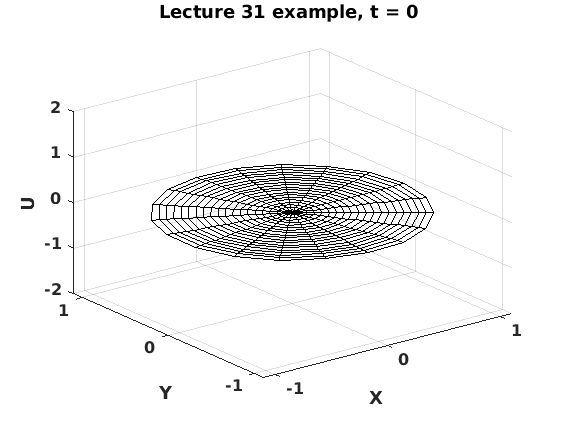
\includegraphics[width=2in]{lec31-1.png}}
\subfloat[]{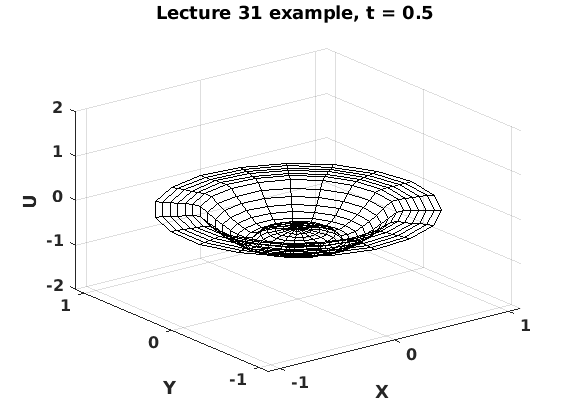
\includegraphics[width=2in]{lec31-2.png}} \\
\subfloat[]{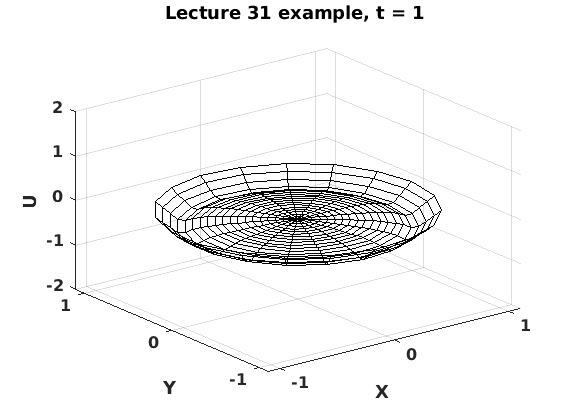
\includegraphics[width=2in]{lec31-3.png}}
\subfloat[]{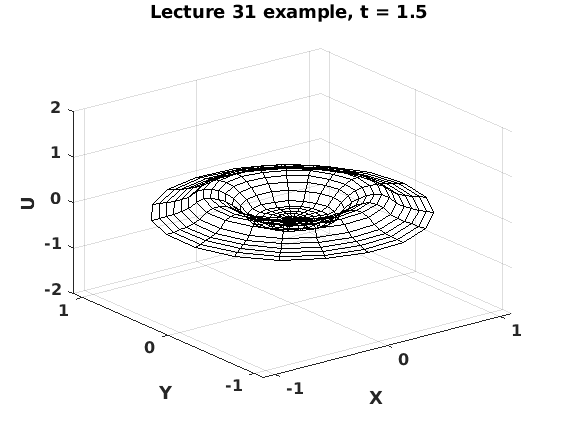
\includegraphics[width=2in]{lec31-4.png}} \\
\subfloat[]{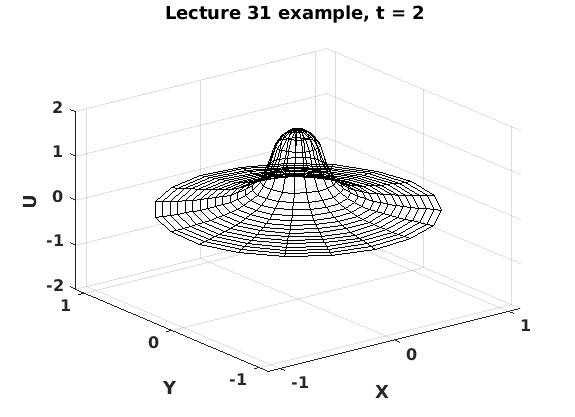
\includegraphics[width=2in]{lec31-5.png}}
\subfloat[]{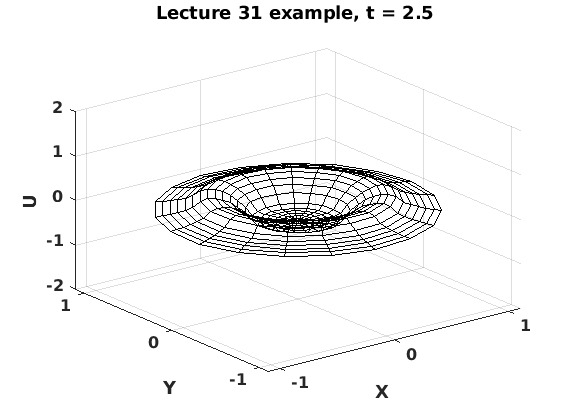
\includegraphics[width=2in]{lec31-6.png}} \\
\subfloat[]{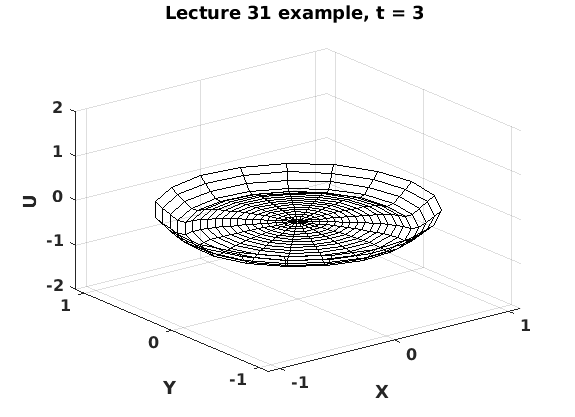
\includegraphics[width=2in]{lec31-7.png}}
\subfloat[]{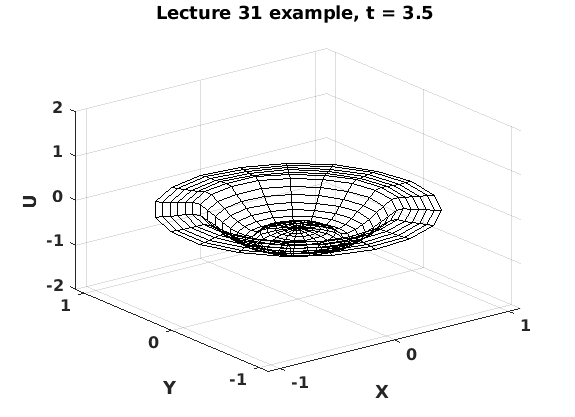
\includegraphics[width=2in]{lec31-8.png}} 
\label{fig:lec31-ex1-plots}
\caption{Plots solution with boundary conditions selected for example 2.}
\end{figure}

